\subsection{Candidate Entity Generation}
\label{sec:candgen}

%To generate the candidate entity table,
We generate candidate English entities for each mention represented in Chinese.
Without a reliable Chinese knowledge base as the bridge,
we use translation tools to produce a set of possible translations of the given mention.
Afterwards, we use several heuristic rules to obtain candidate English entities.
Possible candidate entities consist of:
1) exact match of any mention translation;
2) anchor entities of any mention translation in knowledge base;
3) fuzzy match (e.g., edit distance) of any mention translation. 
Take the Chinese mention ``
%疑犯追踪
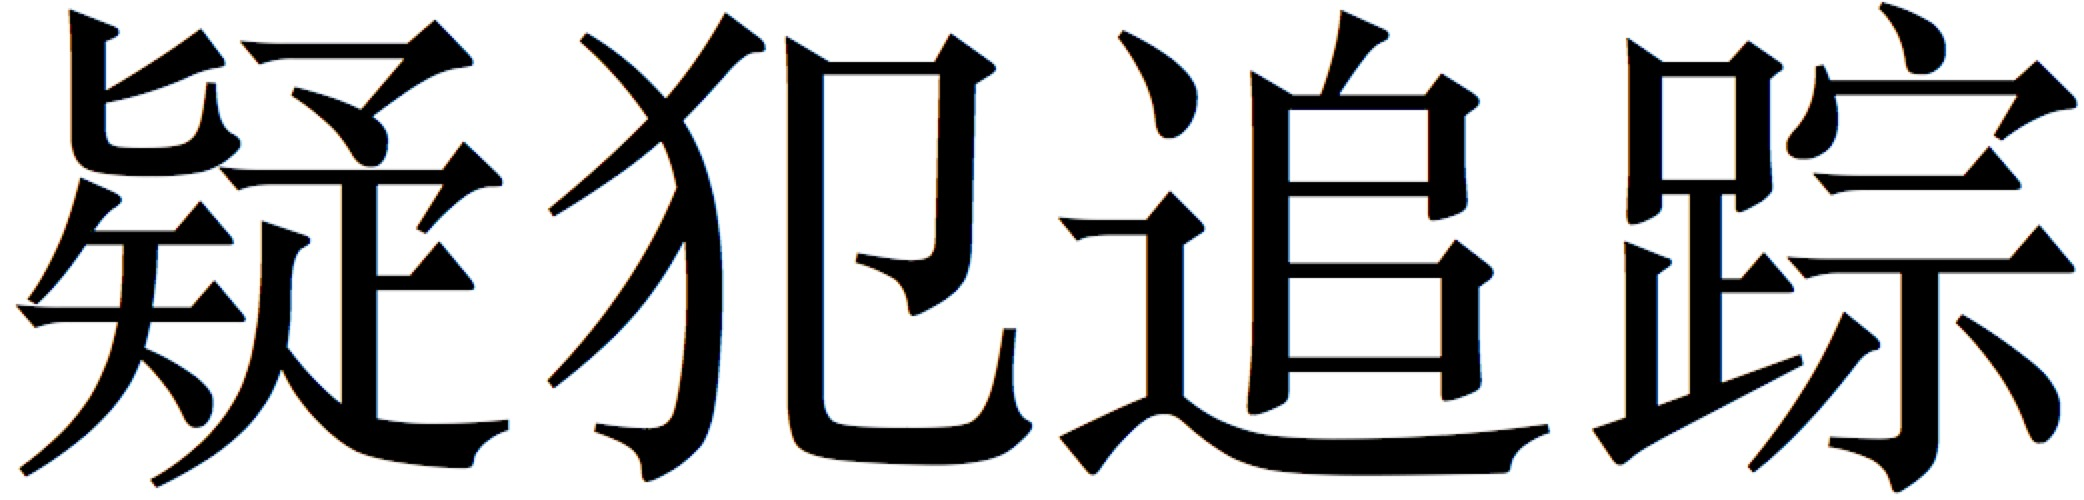
\includegraphics[height=1.3\fontcharht\font`\B]{figures/yifan.png} 
'' as an example,
it can be translated  to ``person of interest'' or  ``suspect tracking'',
depending on what translation tool to use.
The corresponding candidate entity set would contain entities such as
``person of interest'', 
``person of interest (tv series)'' or ``suspect (1987 film)''.
